The purpose of this algorithm is to make a 3D tracking objects, producing position informations 
about the followed target.
These informations will be relevant to define the parameters 
as: the relative velocity, the factor of approaching and of departure.

The proposed algorithm begin with a key image frame where a initial $ROI$ is determined; 
the system then receive a stream of image frames and the tracking system 
enters in looping to follow the target in the frames as is shown in the Fig. \ref{fig:system}.


\begin{figure}[bhp]
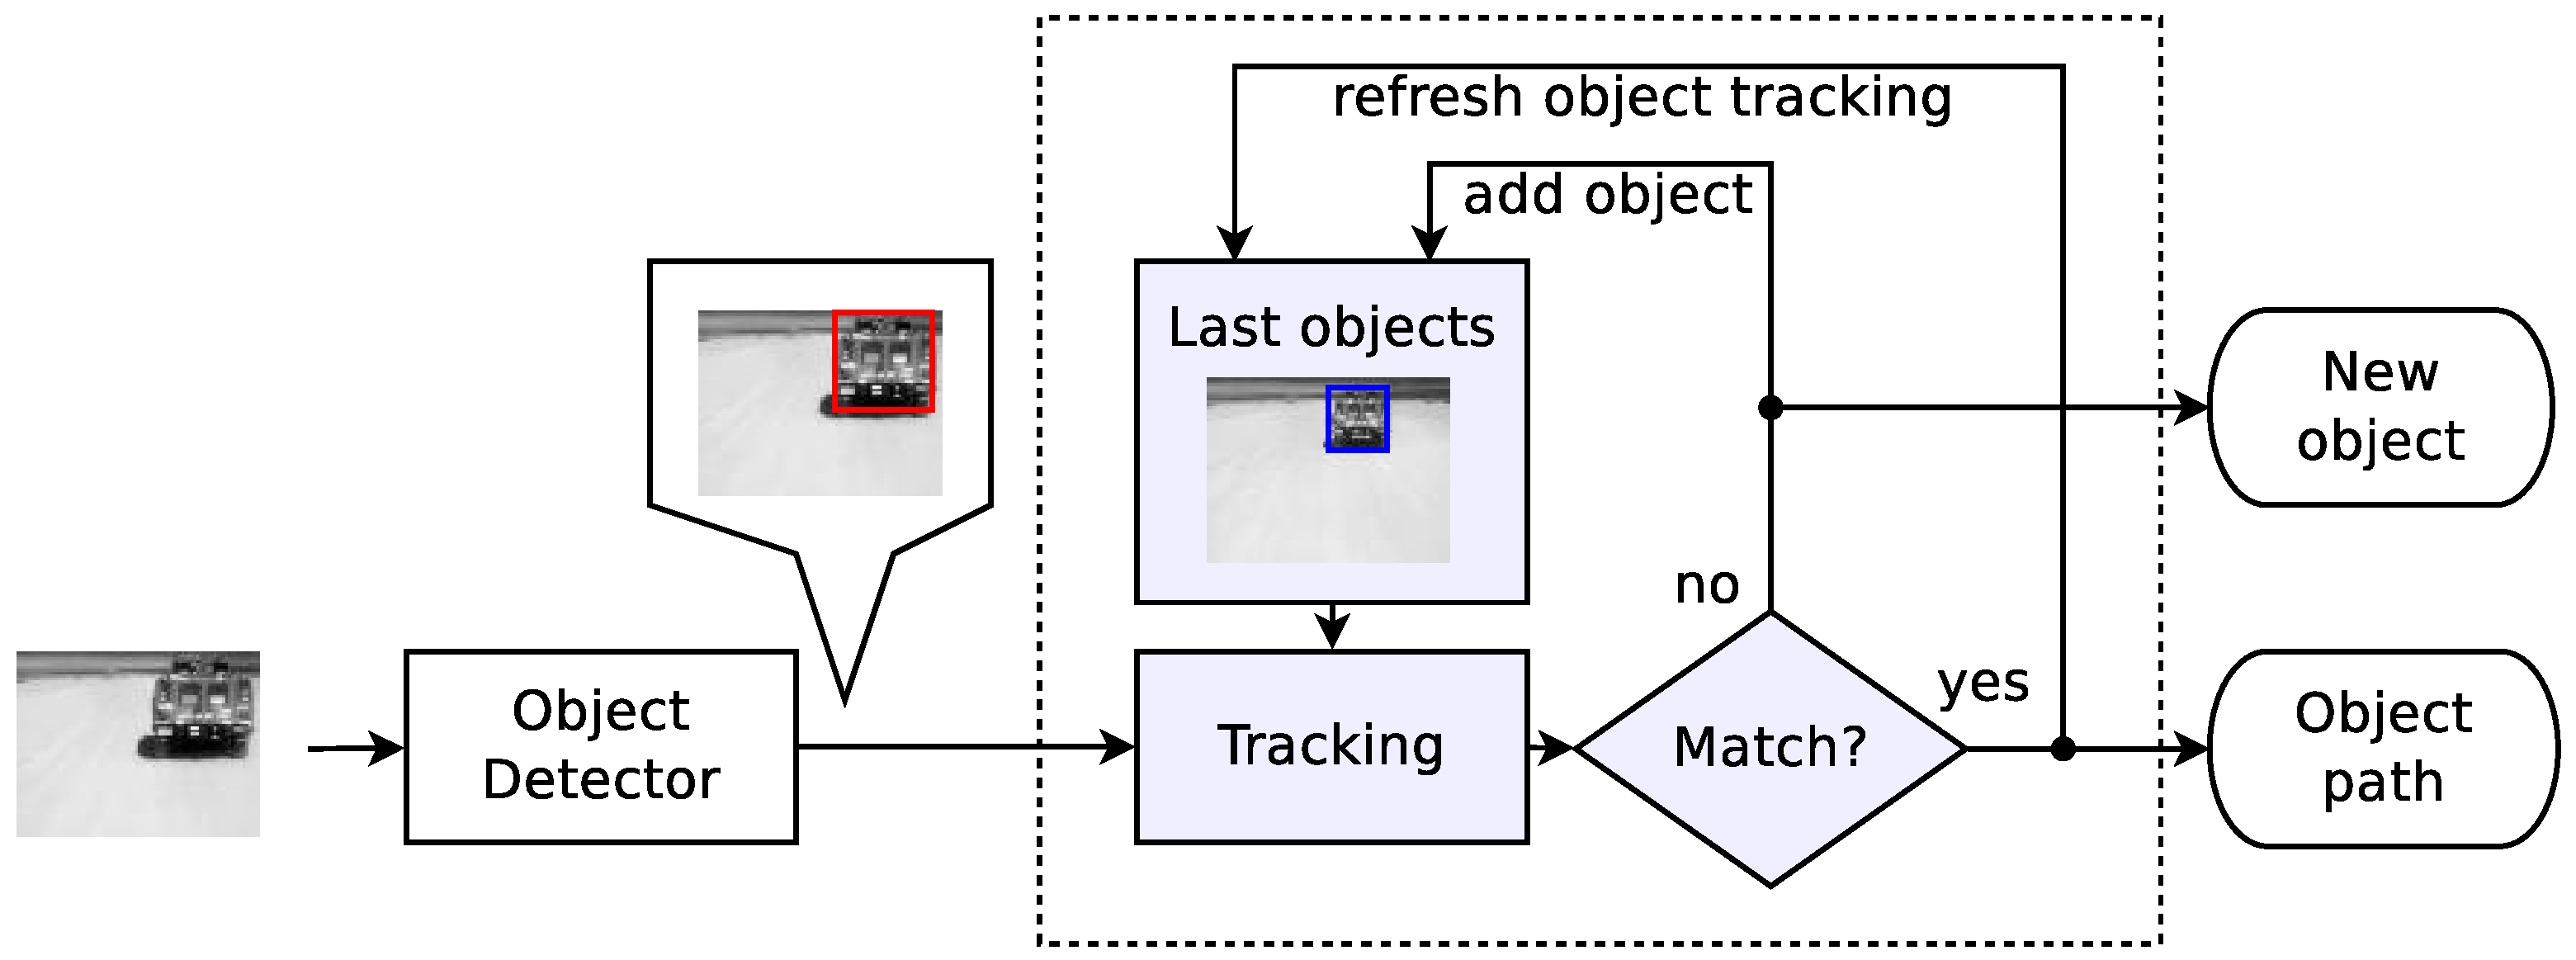
\includegraphics[width=\columnwidth]{images/figure1-diagram1.eps}
\caption{With a current $ROI$ selected, a highest value of $PCC$, between the $ROI$ 
and the Window Of Search (WOS) of next frame, identifies the target; 
the result of search is a displacement vector
between the first and last position of object. 
After, this processing is made again to the next frames.}
\label{fig:system}
\end{figure}

In 2 dimensions, the objects are tracking and given information about its horizontal 
or vertical relative velocity.
When the target moves in 3 dimensions, outputs are the resultant of relative 
velocity and the factor of approaching or departure. 
There isn't a factor in 2 dimensions, since approaching or departure don't exist 
in this situation.

The algorithm developed takes as initial input a key frame with a Region Of 
Interesting ($ROI$) at the position $(x,y,1)$.
Where, $x$ and $y$ represent a position (line and column) in analyzed image,
and $1$ represents the initial deepest position of object in the $ROI$.

%Diagrama1
 %A gente vai explicar o algoritmo como uma caixa fechada , que coisa entra e que coisa sai
 %e os parametros a sintonizar.
 % como usar ele quando implementado, como se fosse uma caixa preta.
